\documentclass[12pt]{article}
\setlength{\oddsidemargin}{0in}
\setlength{\evensidemargin}{0in}
\setlength{\textwidth}{6.5in}
\setlength{\parindent}{0in}
\setlength{\parskip}{\baselineskip}
\usepackage{amsmath,amsfonts,amssymb}
\usepackage{graphicx}
\usepackage[]{algorithmicx}

\usepackage{fancyhdr}
\pagestyle{fancy}

%\usepackage{hyperref}


\setlength{\headsep}{36pt}

\begin{document}

\lhead{{\bf CSCI 3104, Algorithms \\ Explain-It-Back 5} }
\rhead{Name: \fbox{Michael Rogers} \\ ID: \fbox{105667404} \\ {\bf Profs.\ Grochow \& Layer\\ Spring 2019, CU-Boulder}}
\renewcommand{\headrulewidth}{0.5pt}

\phantom{Test} \\ \\
Your social science colleagues are interested in quantifying the differences in
the news sources of ``distant'' groups. Their data is from a social network and
consists of users and their friends. Part of their research involves
quantifying the ``maximum social distance'' of individuals. To accomplish they
need an algorithm that takes in two users as input and returns the maximum
number of social groups that connects them. They propose using a friend of a
friend (FOAF) approach ({\tt foaf()} below) that starts with one of the input
users, finds their FOAFs, then selects the FOAF who has the largest number of
friends in common. For example, in the figure below the user (grey) has four
friends and four FOAFs. One FOAF (black) has 2 friends in common and that user
is selected.  This process repeated for each FOAF until the second input user
is one of the FOAFs. We can assume that a path between any two users exists.
% ----- FIGURE -----
\begin{figure}[h!]
\begin{center}
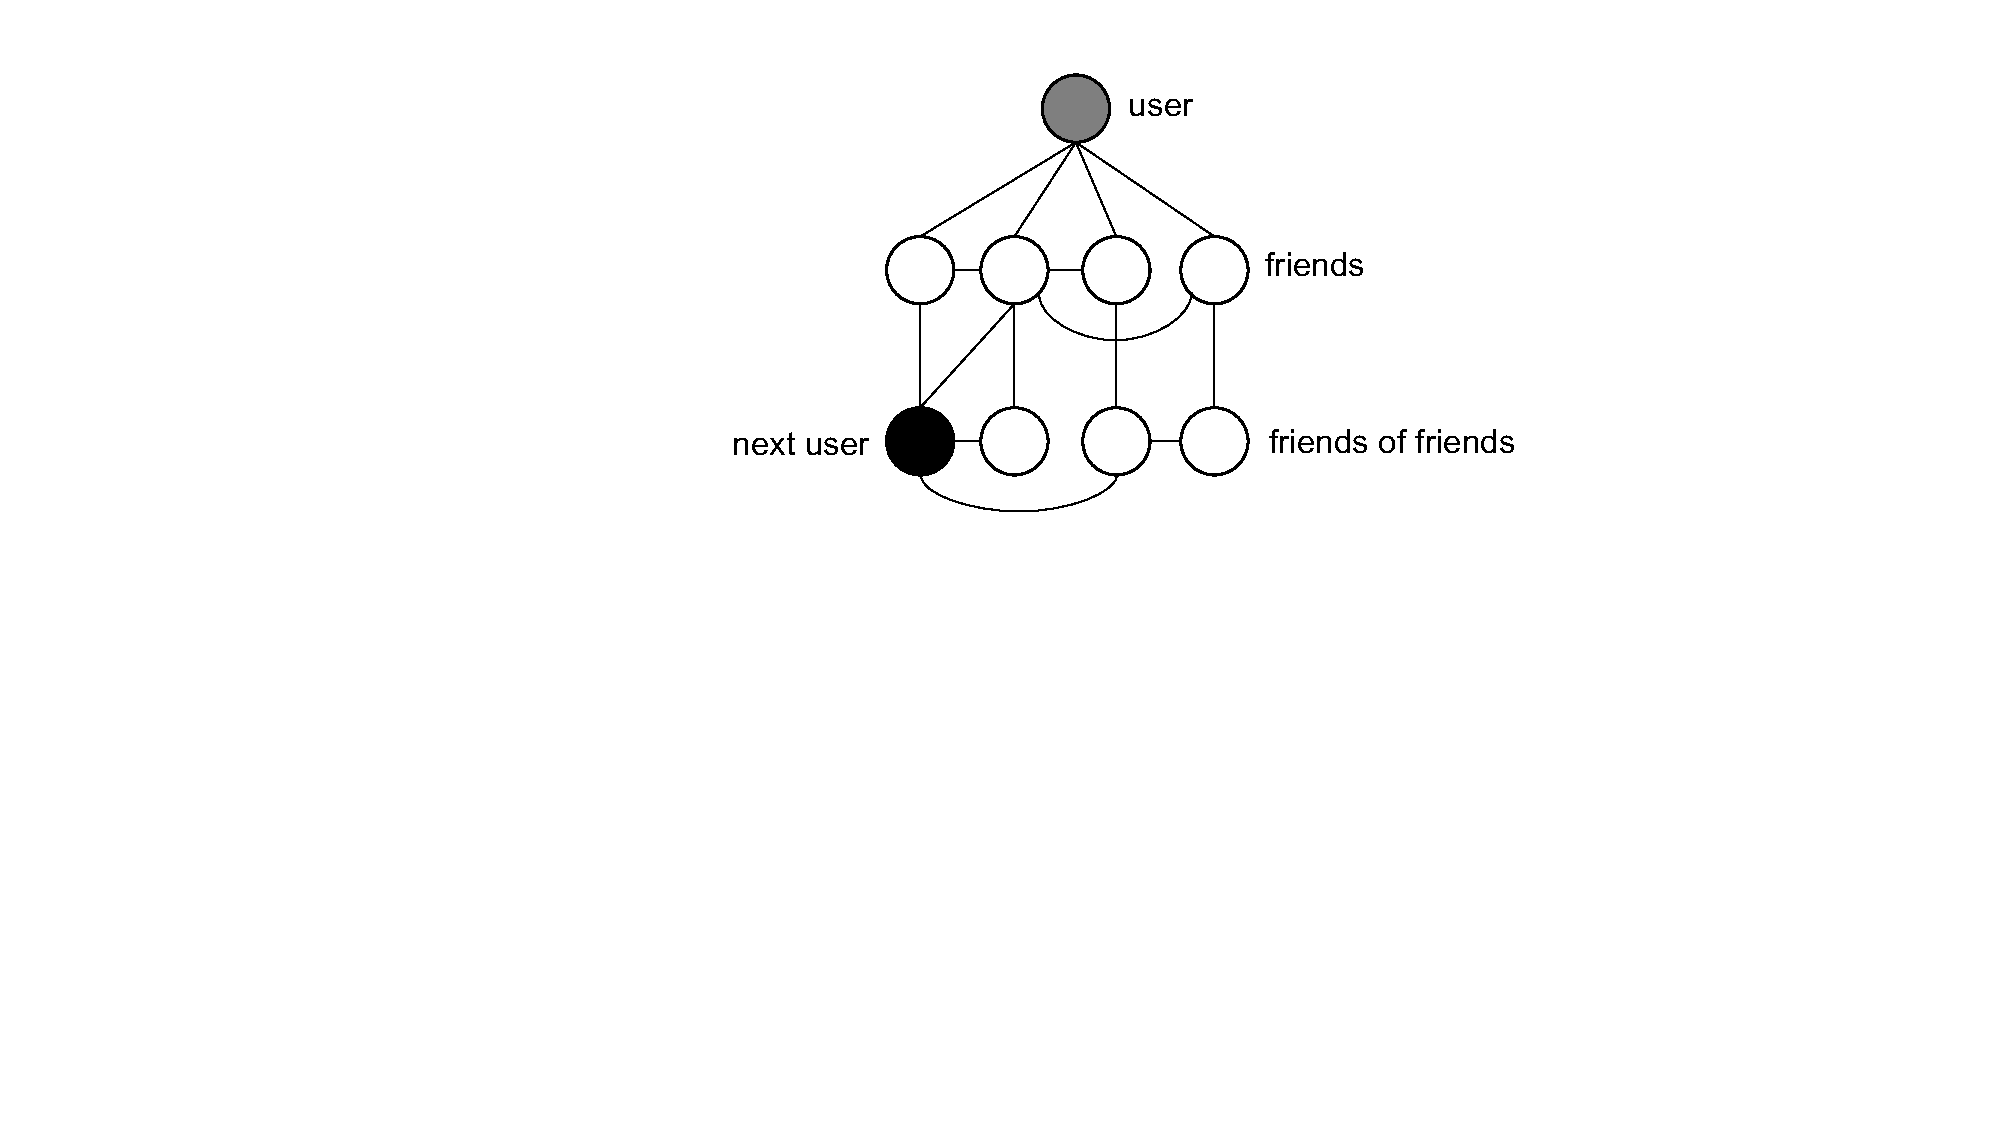
\includegraphics[scale=0.5]{EIB6_graph.pdf}
%An undirected graph representing a triangle: $V=\{1,2,3\}$ and $E=\{(1,2),(1,3),(2,3)\}$
\end{center}
\end{figure}
% ----------
\begin{small}
\begin{verbatim}
foaf(user_1, user_2, d):
  F = friends(user_1) // set user who are friends with user_1
  if user_2 is in F: return d
  FOAF = []
  for f in F:
    if user_2 is in friends(f): return d
    FOAF.append(friends(f) - F) // set subtraction
  max_foaf_count = 0
  max_foaf = NULL
  for f in FOAF:
    foaf_count = | intersect(F,friends(f)) |
    if max_foaf_count < foaf_count:
      max_foaf_count = foaf_count
      max_foaf = f
  foaf(max_foaf, user_2, d+1)
\end{verbatim}
\end{small}
\pagebreak
They seem surprised that, while the algorithm is very fast and give reasonable
results in most cases, every once in a while the algorithm returns a distance
that is different than they expected. Help them understand what assumptions
required for the algorithm they developed and why those are not met here.

\pagebreak

\newpage
\mbox{Hello Social Science colleagues,}
\\ \\ This is a very interesting subject that you are seeking to learn more about. I am happy to help resolve some of the discrepancies in the results that you are seeing. Let me first say that this algorithm that you guys have come up with is very impressive and it makes sense that it is very fast. My understanding is that, although the algorithm is very fast in finding a distance, it is sometimes not outputting the correct maximum distance. I think that I can shed some light on this issue. Assuming you guys understand some basics of algorithms and computer science based on the algorithm you sent me, I may not elaborate on basic computer science concepts. If you have any questions about something I didn't fully explain feel free to ask me. Continuing, while your algorithm is very efficient in looking through these FOAF groups, this is an algorithm called a greedy algorithm. A greedy algorithm is a method that picks the best possible scenario at each step throughout the process. In this case, at every level of friends, it picks the friend with the most amount of FOAF and then follows that tree down until it finds user 2. Greedy algorithms can be correct and can find the result we are looking for very quickly, but they tend to not take the most optimal overall branch because it gets fooled by a step. These algorithms don't have a bigger view of the whole problem, they have tunnel vision. To correct this, we need to look at some baseline assumptions. For this algorithm to be correct, we would need every step to lead to the maximum FOAF. As we can see, that isn't always true. This is the biggest reason that you are getting back some incorrect results from the algorithm. Instead of the algorithm only looking one level behind and in front of itself, we need it to be able to see the whole problem. In other words, we need to dispose of the tunnel vision nature that comes along with greedy algorithms. We can correct this using a method called dynamic programming. Dynamic programming has a similar greedy nature, however instead of having the tunnel vision, this strategy can see the problem as a whole and make a better decision at each step. This will solve these errors you have been seeing in your results. If you need any help implementing this new strategy, feel free to reach out to me, and I would be happy to go into more detail.

Good luck, \\
A Computer Scientist you know 


\newpage
\pagebreak
\end{document}
